\chapter{การออกแบบระบบและรายละเอียดการพัฒนา}
\label{chapter:experiment}

\section{ภาพรวมของเว็บแอพพลิเคชั่น}

เว็บแอพพลิเคชั่นประเมินความสามารถเบื้องต้นของผู้สมัครงาน คือระบบที่จะช่วยให้คัดกรองผู้คนได้มีประสิทธิภาพมากยื่งขึ้น ผ่านการทำข้อสอบที่สามารถกำหนดระดับความยากของข้อสอบได้ และดึงคลังคำถามมาแบบสุ่ม ส่งให้ผู้ทำข้อสอบโดยอัติโนมัติผ่านทางอีเมล เมื่อผู้สมัครงานทำข้อสอบเสร็จแล้ว ข้อสอบจะถูกส่งไปที่ผู้ออก พร้อมตรวจข้อที่เป็นคำถามปลายปิดให้อัตโนมัติ โดยระบบนี้แบ่งเป็น 2 ส่วนหลักๆ คือในส่วนของหน้าบ้านที่ใช้เป็น Vue.js framwork และส่วนของหลังบ้านที่ใช้ Node.js framwork การเก็บข้อมูลทั่วไปถูกเก็บอยู่ใน mongoDB Atlas การเก็บไฟล์ เช่น ไฟล์รูปภาพ หรือไฟล์ต่างๆที่ถูกใช้ในการทำข้อสอบจะถูกเก็บอยู่บน Google Cloud Storage การจัดการอีเมลใช้บริการของ SendGrid เข้ามาช่วยจัดการ และการยืนยันตัวตนจะถูกเข้ารหัสด้วย JOSN Web Token ภาพรวมการทำงานของระบบจะเป็นดังรูป 3.1

\begin{figure}[H]
  \centering
  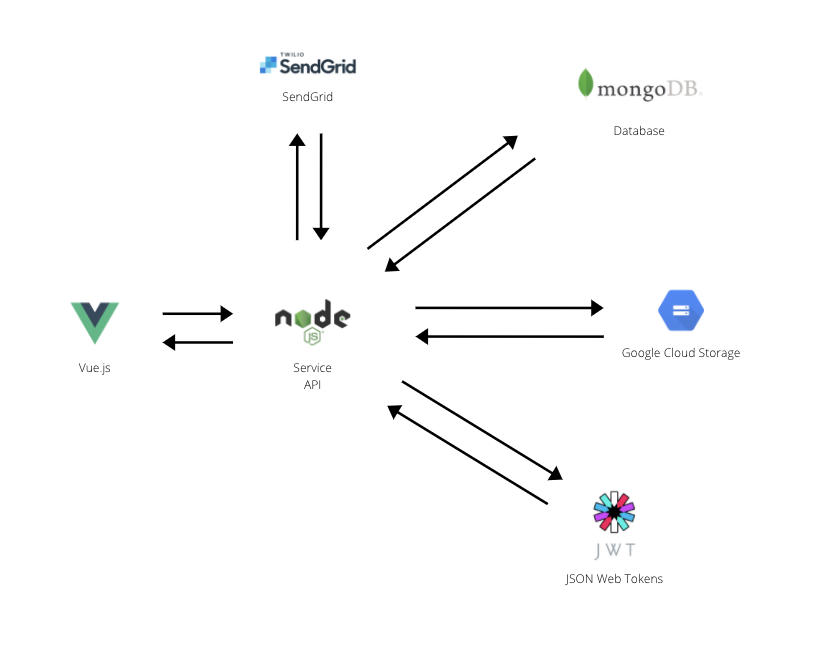
\includegraphics[width=0.9\columnwidth]{ExamaSystem.png}
  \caption{แสดงกระทำงานของระบบประเมินความสามารถเบื้องต้นของผู้สมัครงาน}
  \label{Fig:ExamaSystem}
\end{figure}

\newpage
\section{วิเคราะห์ความต้องการ}

\subsection{ความต้องการที่เป็นหน้าที่หลักของระบบ (Functional Requirement)}
\begin{enumerate}
  \item ผู้ใช้งานสามารถสามารถลงทะเบียนเป็นสมาชิกเพื่อใช้งานเว็บแอพพลิเคชั่นได้  
  \item ผู้ใช้ต้องยืนยันตัวตนผ่านอีเมลหลังจากทำการลงทะเบียน ถึงจะเข้าใช้งานระบบได้
  \item ผู้ใช้งานสามารถสร้าง, แก้ไข และลบหมวดหมู่ข้อสอบได้
  \item ระบบสามารถป้องกันการรีเฟรชเพจและการเปลี่ยนหน้าได้ หากผู้ใช้กำลังสร้างหรือแก้ไขหมวดหมู่ข้อสอบอยุ่
  \item ผู้ใช้งานสามารถยกเลิกการทำข้อสอบได้
  \item ผู้ใช้งานไม่สามารถลบหมวดหมู่ข้อสอบได้ หากถูกใช้งานอยู่ในข้อสอบ
  \item หากหมวดหมู่ข้อสอบถูกส่งไปให้ผู้สมัครงานทำแล้ว หมวดหมู่ข้อสอบนั้นสามารถแก้ไขได้เฉพาะคำตอบเท่านั้น ไม่สามารถแก้ไขคำถามได้
  \item ผู้ใช้งานสามารถสร้างคำถามประเภท ปรนัย, อัตนัย และคำถามที่มีไฟล์แนบได้
  \item คำถามที่เป็นปรนัย สามารถเลือกตอบมากกว่า 1 คำถามได้
  \item สามารถเพิ่มรูปภาพในคำตอบที่เป็นปรนัยได้
  \item ผู้ใช้งานสามารถเปิดหมวดหมู่ข้อสอบให้เป็นสาธารณะได้
  \item หมวดหมู่ข้อสอบที่เป็นสาธารณะ ผู้ที่ไม่ใช้เจ้าของไม่สามารถแก้ไขได้ แต่ระบบสามารถคัดลอกหมวดหมู่ข้อสอบสาธารณะไปเป็นเป็นของตนเองได้ หากผู้ที่ไม่ใช้เจ้าของต้องการทำการแก้ไข
  \item ผู้ใช้งานสามารถค้นหาหมวดหมู่ข้อสอบได้
  \item ผู้ใช้งานสามารถสร้างข้อสอบ ที่กำหนดหมวดหมู่ข้อสอบที่ต้องการเลือกคำถาม,จำนวนข้อ และความยากได้ โดยข้อสอบจะทำการสุ่มเมื่อผู้ใช้ส่งให้ผู้ทำข้อสอบ
  \item ผู้ใช้สามารถลบแก้ไขหมวดหมู่ข้อสอบที่ใช้ จำนวนข้อ และระดับความยากของข้อสอบได้
  \item ผู้ใช้สามารถค้นหาข้อสอบได้
  \item ผู้ใช้สามารถเปิดข้อสอบให้เป็นสาธารณะได้
  \item ข้อสอบที่เป็นสาธารณะ ผู้ที่ไม่ใช้เจ้าของไม่สามารถแก้ไขได้ โดยระบบสามารถคัดลอกข้อสอบสาธารณะไปเป็นเป็นของตนเองได้ หากผู้ที่ไม่ใช้เจ้าของต้องการทำการแก้ไข
  \item ผู้ใช้สามารถกำหนดระยะเวลาในการทำข้อสอบได้
  \item ผู้ใช้สามารถกำหนดวันหมดอายุของข้อสอบได้
  \item ผู้ใช้สามารถส่งข้อสอบให้ผู้สมัครงานด้วยอีเมลผ่านเว็บแอพพลิเคชั่นได้
  \item ผู้ทำข้อสอบสามารถเข้ามาทำข้อสอบในเว็บแอพพลิเคชั่นได้ตลอด หากเวลาในการทำข้อสอบยังไม่หมด
  \item เมื่อผู้ทำข้อสอบทำการส่งข้อสอบแล้ว ระบบสามารถตรวจข้อสอบที่เป็นปรนัยได้
  \item มีการแสดงสถานะบอกว่าผู้ใช้งาน ตรวจข้อสอบนั้นหรือยัง
  \item มีการสรุปคะแนนรวมข้อผู้สมัครงาน
\end{enumerate}

\newcolumntype{L}[1]{>{\raggedright\let\newline\\\arraybackslash}p{#1}}

\section{การวิเคราะห์และออกแบบระบบ}

\subsection{แผนภาพยูสเคส (Use Case Diagram)}

\begin{figure}[H]
  \centering
  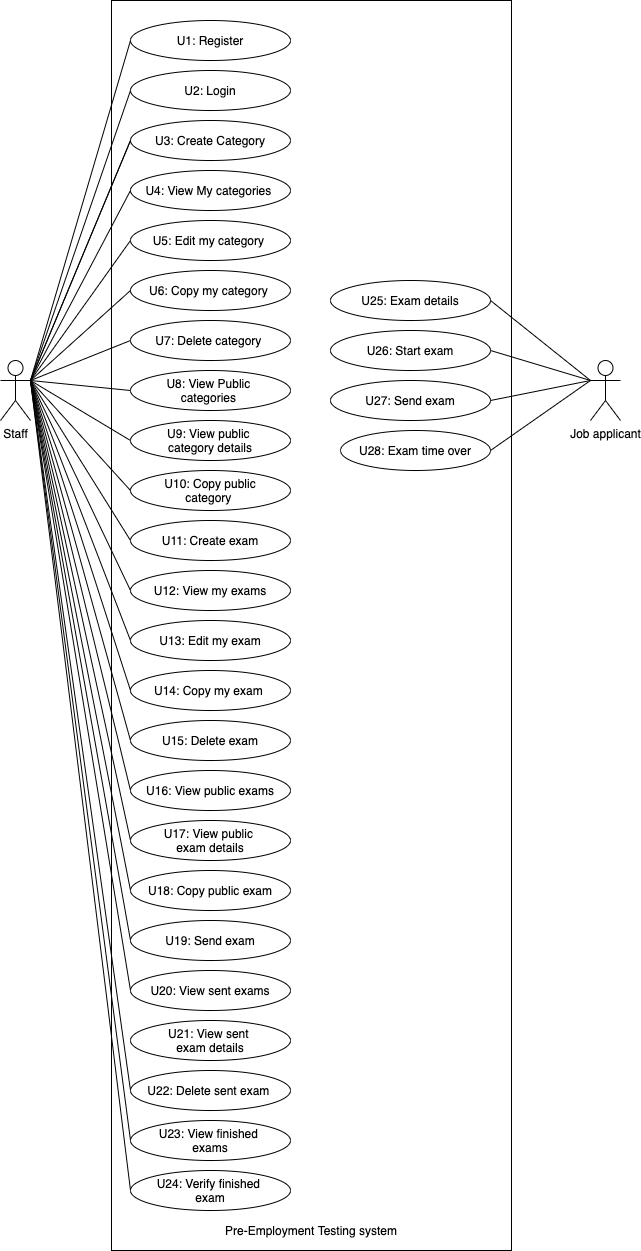
\includegraphics[width=0.8\columnwidth]{examaUseCaseDiagram.png}
  \caption{แผนภาพยูสเคสของระบบ}
  \label{Fig:examaUseCaseDiagram}
\end{figure}

\subsection{รายละเอียดการทำงานในแต่ละยูสเคศ (Use Case Description)}

\subsubsection{รายละเอียดยูสเคส ลงทะเบียน}

\begin{table}[H]
  \begin{tabular}{|l|l|l|} 
  \hline
  Use Case No:                                      & \multicolumn{2}{l|}{1}\\ 
  \hline
  Use Case Name:                                    & \multicolumn{2}{l|}{ลงทะเบียน}\\
  \hline
  Use Case~Scenario:                                & \multicolumn{2}{l|}{ผู้ใช้ลงทะเบียนกับระบบ}\\ 
  \hline
  \vcell{Triggering Event:}                         & \multicolumn{2}{l|}{\vcell{\begin{tabular}[b]{@{}l@{}}เมื่อผู้ใช้เข้าใช้งานเป็นครั้งแรก\end{tabular}}}\\[-\rowheight]
  \printcelltop                                     & \multicolumn{2}{l|}{\printcellmiddle}\\
  \hline
  Brief Description:                                & \multicolumn{2}{l|}{สำหรับให้ผู้ใช้ลงทะเบียนเข้าสู้ระบบ}\\ 
  \hline
  Actors:                                           & \multicolumn{2}{l|}{พนักงาน}\\ 
  \hline
  Related Use Cases:                                & \multicolumn{2}{l|}{-}\\ 
  \hline
  Stakeholders:                                     & \multicolumn{2}{l|}{-}\\ 
  \hline
  Pre - Conditions:                                 & \multicolumn{2}{l|}{-}\\ 
  \hline
  Post - Conditions:                                & \multicolumn{2}{l|}{ผู้ใช้สามารถเข้าใช้งานระบบได้}\\ 
  \hline
  Flow of Events:                                   & \multicolumn{1}{c|}{ผู้ใช้} & \multicolumn{1}{c|}{ระบบ}\\  
  \cline{2-3}
                                                    & \vcell{\begin{tabular}[b]{m{0.28\linewidth}}
                                                      1.ผู้ใช้เลือกลงทะเบียน\\\\\\
                                                      3.ผู้ใช้ทำการกรอกชื่อ-\\นามสกุล,อีเมล,รหัสผ่าน \\และยืนยันรหัสผ่าน แล้ว\\ทำการคลิกลงทะเบียน\\\\\\
                                                      5.ผู้ใช้งานได้รับอีเมล แล้ว\\ทำการคลิกลิงค์เว็บไซต์\\\\\\\\
                                                      \end{tabular}}
                                                    & \vcell{\begin{tabular}[b]{m{0.28\linewidth}}
                                                      \\
                                                      2.ระบบแสดงแบบฟอร์มให้กรอกข้อมูล\\\\\\\\\\
                                                      4.ระบบทำการส่งอีเมลให้ผู้ใช้เพื่อทำการยืนยันอีเมล\\\\\\
                                                      6.ระบบทำการยืนยันอีเมล\\ แล้วแสดงหน้าจอหลักของผู้ใช้งาน
                                                      \end{tabular}}\\[-\rowheight]
                                                    & \printcelltop & \printcelltop\\ 
  \hline
  \vcell{Exception Conditions:}                     & \multicolumn{2}{l|}{\vcell{\begin{tabular}[b]{@{}l@{}}- ผู้ใช้กรอกรายละเอียดไม่ครบถ้วน หรือไม่ตรงเงื่อนไข\\- ผู้ใช้ไม่ได้ทำการยืนยันอีเมล\\- ผู้ใช้กรอกอีเมลที่ไม่มีอยู่จริง\\- ผู้ใช้กรอกออีเมลที่ผู้ใช้งานไม่สามารถเข้าใช้อีเมลนั้นได้\end{tabular}}}\\[-\rowheight]
  \printcelltop                                     & \multicolumn{2}{l|}{\printcellmiddle}\\
  \hline
  \end{tabular}
  \caption{รายละเอียดยูสเคส ลงทะเบียน}
  \label{Table:register}
\end{table}

\subsubsection{รายละเอียดยูสเคส เข้าสู่ระบบ}

\begin{table}[H]
  \begin{tabular}{|l|l|l|} 
  \hline
  Use Case No:                                      & \multicolumn{2}{l|}{2}\\ 
  \hline
  Use Case Name:                                    & \multicolumn{2}{l|}{เข้าสู่ระบบ}\\
  \hline
  Use Case~Scenario:                                & \multicolumn{2}{l|}{ผู้ใช้ต้องการเข้าสู่ระบบ}\\ 
  \hline
  \vcell{Triggering Event:}                         & \multicolumn{2}{l|}{\vcell{\begin{tabular}[b]{@{}l@{}}- เมื่อผู้ใช้ต้องการเข้าใช้งานระบบ\\- ผู้ใช้เข้าเว็ปแอพพลิเคชั่นโดยที่ยังไม่เข้าใช้งานระบบ\end{tabular}}}\\[-\rowheight]
  \printcelltop                                     & \multicolumn{2}{l|}{\printcellmiddle}\\
  \hline
  Brief Description:                                & \multicolumn{2}{l|}{สำหรับให้ผู้ใช้เข้าสู่ระบบเพื่อเข้าใช้งานเว็ปแอปพลิเคชั่น}\\ 
  \hline
  Actors:                                           & \multicolumn{2}{l|}{พนักงาน}\\ 
  \hline
  Related Use Cases:                                & \multicolumn{2}{l|}{ลงทะเบียน}\\ 
  \hline
  Stakeholders:                                     & \multicolumn{2}{l|}{-}\\ 
  \hline
  Pre - Conditions:                                 & \multicolumn{2}{l|}{ผู้ใช้ต้องทำการลงทะเบียนและยืนยันตัวตนผ่านอีเมลเรียบร้อยแล้ว}\\ 
  \hline
  Post - Conditions:                                & \multicolumn{2}{l|}{ระบบแสดงหน้าจอสำหรับผู้ใช้งาน}\\ 
  \hline
  Flow of Events:                                   & \multicolumn{1}{c|}{ผู้ใช้} & \multicolumn{1}{c|}{ระบบ}\\  
  \cline{2-3}
                                                    & \vcell{\begin{tabular}[b]{m{0.28\linewidth}}
                                                      1.ผู้ใช้เข้าหน้าเว็ปโดยที่ยังไม่ได้ทำการเข้าสู้ระบบ\\\\\\
                                                      3.ผู้ใช้ทำการกรอกอีเมล และรหัสผ่านแล้วทำการคลิกเข้าสู่ระบบ หรือกด Enter บนแป้นพิมพ์\\\\\\
                                                      \end{tabular}}
                                                    & \vcell{\begin{tabular}[b]{m{0.28\linewidth}}
                                                      \\\\
                                                      2.ระบบแสดงแบบฟอร์มให้กรอกข้อมูล\\\\\\\\\\
                                                      4.ระบบแสดงหน้าจอหลักของผู้ใช้งาน
                                                      \end{tabular}}\\[-\rowheight]
                                                    & \printcelltop & \printcelltop\\ 
  \hline
  \vcell{Exception Conditions:}                     & \multicolumn{2}{l|}{\vcell{\begin{tabular}[b]{@{}l@{}}ผู้ใช้กรอกอีเมล หรือรหัสผ่านผิด\end{tabular}}}\\[-\rowheight]
  \printcelltop                                     & \multicolumn{2}{l|}{\printcellmiddle}\\
  \hline
  \end{tabular}
  \caption{รายละเอียดยูสเคส เข้าสู่ระบบ}
  \label{Table:login}
\end{table}

\subsubsection{รายละเอียดยูสเคส สร้างหมวดหมู่ของข้อสอบ}

\begin{table}[H]
  \begin{tabular}{|l|l|l|} 
  \hline
  Use Case No:                                      & \multicolumn{2}{l|}{3}\\ 
  \hline
  Use Case Name:                                    & \multicolumn{2}{l|}{สร้างหมวดหมู่ของข้อสอบ}\\
  \hline
  Use Case~Scenario:                                & \multicolumn{2}{l|}{ผู้ใช้ต้องการสร้างหมวดหมู่ของข้อสอบ}\\ 
  \hline
  \vcell{Triggering Event:}                         & \multicolumn{2}{l|}{\vcell{\begin{tabular}[b]{@{}l@{}}เมื่อผู้ใช้ต้องการสร้างหมวดหมู่ของข้อสอบ ไว้ใช้ในข้อสอบของ\\ตนเอง หรือให้พนักงานคนอื่นใช้\end{tabular}}}\\[-\rowheight]
  \printcelltop                                     & \multicolumn{2}{l|}{\printcellmiddle}\\
  \hline
  \vcell{Brief Description:}                        & \multicolumn{2}{l|}{\vcell{\begin{tabular}[b]{@{}l@{}}สำหรับให้ผู้ใช้ ออกข้อสอบโดยแบ่งแยกตามแต่ละหมวดหมู่ เช่น\\คณิตศาสตร์, โปรแกรมมิ่ง หรือ แบบทดสอบสติปัญญา โดยมีชนิด\\คำถามแบ่งออกเป็น อัตนัย, ปรนัย และคำถามที่มีไฟล์แนบ\end{tabular}}}\\[-\rowheight]
  \printcelltop                                     & \multicolumn{2}{l|}{\printcellmiddle}\\
  \hline
  Actors:                                           & \multicolumn{2}{l|}{พนักงาน}\\ 
  \hline
  Related Use Cases:                                & \multicolumn{2}{l|}{เข้าสู่ระบบ}\\ 
  \hline
  Stakeholders:                                     & \multicolumn{2}{l|}{-}\\ 
  \hline
  Pre - Conditions:                                 & \multicolumn{2}{l|}{ผู้ใช้ต้องทำการเข้าสู่ระบบ}\\ 
  \hline
  \vcell{Post - Conditions:}                        & \multicolumn{2}{l|}{\vcell{\begin{tabular}[b]{@{}l@{}}ผู้ใช้มีหมวดหมู่ของข้อสอบที่ตนเองสร้างขึ้น และแสดงหน้าหมวด\\หมู่ทั้งหมดของผู้ใช้\end{tabular}}}\\[-\rowheight]
  \printcelltop                                     & \multicolumn{2}{l|}{\printcellmiddle}\\
  \hline
  Flow of Events:                                   & \multicolumn{1}{c|}{ผู้ใช้} & \multicolumn{1}{c|}{ระบบ}\\  
  \cline{2-3}
                                                    & \vcell{\begin{tabular}[b]{m{0.28\linewidth}}
                                                      1.ไปที่หน้าสร้างหมวดหมู่\\\\\\
                                                      3.ผู้ใช้กรอกชื่อหมวดหมู่\\และกรอกหัวเรื่อง\\
                                                      4.สร้างคำถามภายใต้ หมวดหมู่นั้นโดยสามารถเลือก\\ระดับความยาก และประเภทของคำถาม แล้วทำการคลิกสร้างหมวดหมู่\\\\\\\\\\                                                 
                                                      \end{tabular}}
                                                    & \vcell{\begin{tabular}[b]{m{0.28\linewidth}}
                                                      \\
                                                      2.ระบบแสดงหน้าสร้าง\\หมวดหมู่ของข้อสอบ\\\\\\\\\\\\\\\\
                                                      5.ระบบทำการสร้างหมดหมู่ของข้อสอบ แล้วแสดงหน้าหมวดหมู่ข้อสอบทั้งหมด\\ของผู้ใช้
                                                      \end{tabular}}\\[-\rowheight]
                                                    & \printcelltop & \printcelltop\\ 
  \hline
  \vcell{Exception Conditions:}                     & \multicolumn{2}{l|}{\vcell{\begin{tabular}[b]{@{}l@{}}- ผู้ใช้กรอกขื่อหมวดหมู่ซ้ำกับ หมวดหมู่ที่ตนเองมีอยู่แล้ว\\- ผู้ใช้กรอกข้อมูลไม่ครบ ตามฟอร์มที่ให้กรอก\\- ไฟล์ที่แนบมามีขนาดใหญ่เกินที่กำหนด หรือประเภทของไฟล์ไม่\\\hspace{0.22cm}ถูกต้อง\end{tabular}}}\\[-\rowheight]
  \printcelltop                                     & \multicolumn{2}{l|}{\printcellmiddle}\\
  \hline
  \end{tabular}
  \caption{รายละเอียดยูสเคส สร้างหมวดหมู่ของข้อสอบ}
  \label{Table:createCategory}
\end{table}

\subsubsection{รายละเอียดยูสเคส ดูหมวดหมู่ข้อสอบของผู้ใช้}

\begin{table}[H]
  \begin{tabular}{|l|l|l|} 
  \hline
  Use Case No:                                      & \multicolumn{2}{l|}{4}\\ 
  \hline
  Use Case Name:                                    & \multicolumn{2}{l|}{ดูหมวดหมู่ข้อสอบของผู้ใช้}\\
  \hline
  Use Case~Scenario:                                & \multicolumn{2}{l|}{ผู้ใช้ต้องการดูหมวดหมู่ข้อสอบของตนเอง}\\ 
  \hline
  \vcell{Triggering Event:}                         & \multicolumn{2}{l|}{\vcell{\begin{tabular}[b]{@{}l@{}}- เมื่อผู้ใช้ต้องการดูหมวดหมู่ของข้อสอบของตนเอง\\- เมื่อผู้ใช้สร้างประเภทของข้อสอบสำเร็จ หน้าเว็ปจะทำการไป\\\hspace{0.22cm}แสดงผลที่หน้าหมวดหมู่ข้อสอบทั้งหมเของผู้ใช้\end{tabular}}}\\[-\rowheight]
  \printcelltop                                     & \multicolumn{2}{l|}{\printcellmiddle}\\
  \hline
  \vcell{Brief Description:}                        & \multicolumn{2}{l|}{\vcell{\begin{tabular}[b]{@{}l@{}}สำหรับให้ผู้ใช้งานดูหมวดหมู่ของข้อสอบที่ตนเองสร้างขึ้น หรือ\\หมวดหมู่ที่ไปคัดลอกมาจากหมวดหมู่สาธารณะ\end{tabular}}}\\[-\rowheight]
  \printcelltop                                     & \multicolumn{2}{l|}{\printcellmiddle}\\
  \hline
  Actors:                                           & \multicolumn{2}{l|}{พนักงาน}\\ 
  \hline
  \vcell{Related Use Cases:}                        & \multicolumn{2}{l|}{\vcell{\begin{tabular}[b]{@{}l@{}}เข้าสู่ระบบ, สร้างหมวดหมู่ของข้อสอบ, คัดลอกหมวดหมู่ข้อสอบ\\จากหมวดหมู่ข้อสอบสาธารณะ\end{tabular}}}\\[-\rowheight]
  \printcelltop                                     & \multicolumn{2}{l|}{\printcellmiddle}\\
  \hline
  Stakeholders:                                     & \multicolumn{2}{l|}{-}\\ 
  \hline
  \vcell{Pre - Conditions:}                         & \multicolumn{2}{l|}{\vcell{\begin{tabular}[b]{@{}l@{}}- ผู้ใช้ต้องทำการเข้าสู่ระบบ\\- สร้างหมวดหมู่ของข้อสอบ หรือคัดลอกหมวดหมู่ข้อสอบจาก\\\hspace{0.22cm}หมวดหมู่ข้อสอบสาธารณะ\end{tabular}}}\\[-\rowheight]
  \printcelltop                                     & \multicolumn{2}{l|}{\printcellmiddle}\\
  \hline
  \vcell{Post - Conditions:}                        & \multicolumn{2}{l|}{\vcell{\begin{tabular}[b]{@{}l@{}}แสดงหน้าหมวดหมู่ทั้งหมดของผู้ใช้\end{tabular}}}\\[-\rowheight]
  \printcelltop                                     & \multicolumn{2}{l|}{\printcellmiddle}\\
  \hline
  Flow of Events:                                   & \multicolumn{1}{c|}{ผู้ใช้} & \multicolumn{1}{c|}{ระบบ}\\  
  \cline{2-3}
                                                    & \vcell{\begin{tabular}[b]{m{0.28\linewidth}}
                                                      1.ไปที่หน้าดูหมวดหมู่ข้อ\\สอบของผู้ใช้                                            
                                                      \end{tabular}}
                                                    & \vcell{\begin{tabular}[b]{m{0.28\linewidth}}
                                                      \\\\
                                                      2.ระบบแสดงหมวดหมู่\\ทั้งหมดของผู้ใช้
                                                      \end{tabular}}\\[-\rowheight]
                                                    & \printcelltop & \printcelltop\\ 
  \hline
  \vcell{Exception Conditions:}                     & \multicolumn{2}{l|}{\vcell{\begin{tabular}[b]{@{}l@{}}ผู้ใช้ไม่มีหมวดหมู่ข้อสอบ\end{tabular}}}\\[-\rowheight]
  \printcelltop                                     & \multicolumn{2}{l|}{\printcellmiddle}\\
  \hline
  \end{tabular}
  \caption{รายละเอียดยูสเคส ดูหมวดหมู่ข้อสอบของผู้ใช้}
  \label{Table:viewMyCategory}
\end{table}

\subsubsection{รายละเอียดยูสเคส แก้ไขหมวดหมู่ข้อสอบของผู้ใช้}

\begin{table}[H]
  \begin{tabular}{|l|l|l|} 
  \hline
  Use Case No:                                      & \multicolumn{2}{l|}{5}\\ 
  \hline
  Use Case Name:                                    & \multicolumn{2}{l|}{แก้ไขหมวดหมู่ข้อสอบของผู้ใช้}\\
  \hline
  Use Case~Scenario:                                & \multicolumn{2}{l|}{ผู้ใช้ต้องการแก้ไขหมวดหมู่ข้อสอบของตนเอง}\\ 
  \hline
  \vcell{Triggering Event:}                         & \multicolumn{2}{l|}{\vcell{\begin{tabular}[b]{@{}l@{}}เมื่อผู้ใช้ต้องการแก้ไขรายละเอียดในหมวดหมู่ข้อสอบ เช่นเพิ่มคำ\\ถาม, แก้ไขคำถาม หรือแก้ไขชื่อหมวดหมู่\end{tabular}}}\\[-\rowheight]
  \printcelltop                                     & \multicolumn{2}{l|}{\printcellmiddle}\\
  \hline
  \vcell{Brief Description:}                        & \multicolumn{2}{l|}{\vcell{\begin{tabular}[b]{@{}l@{}}สำหรับให้ผู้ใช้งานแก้ไขรายละเอียดต่างๆในหมวดหมู่ข้อสอบ\end{tabular}}}\\[-\rowheight]
  \printcelltop                                     & \multicolumn{2}{l|}{\printcellmiddle}\\
  \hline
  Actors:                                           & \multicolumn{2}{l|}{พนักงาน}\\ 
  \hline
  \vcell{Related Use Cases:}                        & \multicolumn{2}{l|}{\vcell{\begin{tabular}[b]{@{}l@{}}เข้าสู่ระบบ, สร้างหมวดหมู่ของข้อสอบ, คัดลอกหมวดหมู่ข้อสอบ\\จากหมวดหมู่ข้อสอบสาธารณะ\end{tabular}}}\\[-\rowheight]
  \printcelltop                                     & \multicolumn{2}{l|}{\printcellmiddle}\\
  \hline
  Stakeholders:                                     & \multicolumn{2}{l|}{-}\\ 
  \hline
  \vcell{Pre - Conditions:}                         & \multicolumn{2}{l|}{\vcell{\begin{tabular}[b]{@{}l@{}}- ผู้ใช้ต้องทำการเข้าสู่ระบบ\\- สร้างหมวดหมู่ของข้อสอบ หรือคัดลอกหมวดหมู่ข้อสอบจาก\\\hspace{0.22cm}หมวดหมู่ข้อสอบสาธารณะ\end{tabular}}}\\[-\rowheight]
  \printcelltop                                     & \multicolumn{2}{l|}{\printcellmiddle}\\
  \hline
  \vcell{Post - Conditions:}                        & \multicolumn{2}{l|}{\vcell{\begin{tabular}[b]{@{}l@{}}แสดงหน้าหมวดหมู่ทั้งหมดของผู้ใช้\end{tabular}}}\\[-\rowheight]
  \printcelltop                                     & \multicolumn{2}{l|}{\printcellmiddle}\\
  \hline
  Flow of Events:                                   & \multicolumn{1}{c|}{ผู้ใช้} & \multicolumn{1}{c|}{ระบบ}\\  
  \cline{2-3}
                                                    & \vcell{\begin{tabular}[b]{m{0.28\linewidth}}
                                                      1.ไปที่หน้าดูหมวดหมู่ข้อ\\สอบของผู้ใช้\\\\\\
                                                      3.คลิกที่หมวดหมู่ของ\\ข้อสอบที่ต้องการแก้ไข\\\\\\
                                                      5.ผู้ใช้ทำการแก้ไขข้อมูล\\ต่างๆในประเภทที่ต้องการ\\ แล้วทำการคลิกยืนยันการ\\แก้ไข\\\\\\\\
                                                      \end{tabular}}
                                                    & \vcell{\begin{tabular}[b]{m{0.28\linewidth}}
                                                      \\\\
                                                      2.ระบบแสดงหมวดหมู่\\ทั้งหมดของผู้ใช้\\\\\\
                                                      4.ระบบแสดงหน้าแก้ไข\\หมวดหมู่นั้นๆ\\\\\\\\\\
                                                      6.ระบบทำการแก้ไขข้อมูล\\
                                                      7.ระบบแสดงหน้าหมวดหมู่ทั้งหมดของผู้ใช้\\
                                                      \end{tabular}}\\[-\rowheight]
                                                    & \printcelltop & \printcelltop\\ 
  \hline
  \vcell{Exception Conditions:}                     & \multicolumn{2}{l|}{\vcell{
                                                        \begin{tabular}[b]{@{}l@{}}
                                                          - ผู้ใช้กรอกชื่อหมวดหมู่ซ้ำกับ หมวดหมู่ที่ตนเองมีอยู่แล้ว\\
                                                          - ผู้ใช้กรอกรายละเอียดไม่ครบถ้วน หรือไม่ตรงเงื่อนไข\\
                                                          - ไฟล์ที่แนบมามีขนาดใหญ่เกินที่กำหนด หรือประเภทของไฟล์\\\hspace{0.22cm}ไม่ถูกต้อง\\
                                                          - สามารถแก้ไขได้แค่คำตอบ หากข้อสอบเคยถูกส่งไปแล้ว
                                                        \end{tabular}}}\\[-\rowheight]
  \printcelltop                                     & \multicolumn{2}{l|}{\printcellmiddle}\\
  \hline
  \end{tabular}
  \caption{รายละเอียดยูสเคส แก้ไขหมวดหมู่ข้อสอบของผู้ใช้}
  \label{Table:editMyCategory}
\end{table}

\subsubsection{รายละเอียดยูสเคส คัดลอกหมวดหมู่ข้อสอบของผู้ใช้}

\begin{table}[H]
  \begin{tabular}{|l|l|l|} 
  \hline
  Use Case No:                                      & \multicolumn{2}{l|}{6}\\ 
  \hline
  Use Case Name:                                    & \multicolumn{2}{l|}{คัดลอกหมวดหมู่ข้อสอบของผู้ใช้}\\
  \hline
  Use Case~Scenario:                                & \multicolumn{2}{l|}{ผู้ใช้ต้องการคัดลอกหมวดหมู่ข้อสอบของตนเอง}\\ 
  \hline
  \vcell{Triggering Event:}                         & \multicolumn{2}{l|}{\vcell{\begin{tabular}[b]{@{}l@{}}เมื่อผู้ใช้ต้องการแก้ไขหมวดหมู่ของข้อสอบที่ถูกส่งให้ผู้สมัครงาน\\แล้ว ทำให้ไม่สามารถแก้ไขหมวดหมู่เดิมได้ หรือต้องการคัดลอก\\หมวดหมู่มาแก้ไข โดยที่ไม่ต้องการให้กระทบหมวดหมู่เดิม\end{tabular}}}\\[-\rowheight]
  \printcelltop                                     & \multicolumn{2}{l|}{\printcellmiddle}\\
  \hline
  \vcell{Brief Description:}                        & \multicolumn{2}{l|}{\vcell{\begin{tabular}[b]{@{}l@{}}สำหรับให้ผู้ใช้งานคัดลอกหมวดหมู่ข้อสอบของตนเอง\end{tabular}}}\\[-\rowheight]
  \printcelltop                                     & \multicolumn{2}{l|}{\printcellmiddle}\\
  \hline
  Actors:                                           & \multicolumn{2}{l|}{พนักงาน}\\ 
  \hline
  \vcell{Related Use Cases:}                        & \multicolumn{2}{l|}{\vcell{\begin{tabular}[b]{@{}l@{}}เข้าสู่ระบบ, สร้างหมวดหมู่ของข้อสอบ, ส่งข้อสอบให้ผู้สมัคร\end{tabular}}}\\[-\rowheight]
  \printcelltop                                     & \multicolumn{2}{l|}{\printcellmiddle}\\
  \hline
  Stakeholders:                                     & \multicolumn{2}{l|}{-}\\ 
  \hline
  \vcell{Pre - Conditions:}                         & \multicolumn{2}{l|}{\vcell{\begin{tabular}[b]{@{}l@{}}- ผู้ใช้ต้องทำการเข้าสู่ระบบ\\- สร้างหมวดหมู่ของข้อสอบ หรือคัดลอกหมวดหมู่ข้อสอบจาก\\\hspace{0.22cm}หมวดหมู่ข้อสอบสาธารณะ\end{tabular}}}\\[-\rowheight]
  \printcelltop                                     & \multicolumn{2}{l|}{\printcellmiddle}\\
  \hline
  \vcell{Post - Conditions:}                        & \multicolumn{2}{l|}{\vcell{\begin{tabular}[b]{@{}l@{}}ระบบทำการคัดลอกหมวดหมู่ของข้อสอบที่ผู้ใช้ต้องการ\end{tabular}}}\\[-\rowheight]
  \printcelltop                                     & \multicolumn{2}{l|}{\printcellmiddle}\\
  \hline
  Flow of Events:                                   & \multicolumn{1}{c|}{ผู้ใช้} & \multicolumn{1}{c|}{ระบบ}\\  
  \cline{2-3}
                                                    & \vcell{\begin{tabular}[b]{m{0.28\linewidth}}
                                                      1.ไปที่หน้าดูหมวดหมู่\\ข้อสอบของผู้ใช้\\\\\\
                                                      3.คลิกปุ่มคักลอกที่หมวด\\หมู่ที่ต้องการคัดลอก\\\\\\
                                                      5.ผู้ใช้งานกดยืนยันการคัด\\ลอก\\\\\\
                                                      \end{tabular}}
                                                    & \vcell{\begin{tabular}[b]{m{0.28\linewidth}}
                                                      \\\\
                                                      2.ระบบแสดงหมวดหมู่\\ทั้งหมดของผู้ใช้\\\\\\
                                                      4.ระบบแสดงหน้ายืนยันการคัดลอก\\\\\\
                                                      6.ระบบทำการคัดลอกหมวดหมู่ข้อสอบนั้น\\
                                                      \end{tabular}}\\[-\rowheight]
                                                    & \printcelltop & \printcelltop\\ 
  \hline
  \vcell{Exception Conditions:}                     & \multicolumn{2}{l|}{\vcell{
                                                        \begin{tabular}[b]{@{}l@{}}
                                                          ผู้ใช้ไม่มีหมวดหมู่ข้อสอบ
                                                        \end{tabular}}}\\[-\rowheight]
  \printcelltop                                     & \multicolumn{2}{l|}{\printcellmiddle}\\
  \hline
  \end{tabular}
  \caption{รายละเอียดยูสเคส คัดลอกหมวดหมู่ข้อสอบของผู้ใช้}
  \label{Table:copyMyCategory}
\end{table}

\subsubsection{รายละเอียดยูสเคส ลบหมวดหมู่ข้อสอบของผู้ใช้}

\begin{table}[H]
  \begin{tabular}{|l|l|l|} 
  \hline
  Use Case No:                                      & \multicolumn{2}{l|}{7}\\ 
  \hline
  Use Case Name:                                    & \multicolumn{2}{l|}{ลบหมวดหมู่ข้อสอบของผู้ใช้}\\
  \hline
  Use Case~Scenario:                                & \multicolumn{2}{l|}{ผู้ใช้ต้องการลบหมวดหมู่ข้อสอบของตนเอง}\\ 
  \hline
  \vcell{Triggering Event:}                         & \multicolumn{2}{l|}{\vcell{\begin{tabular}[b]{@{}l@{}}เมื่อผู้ใช้ไม่ต้องการที่จะใช้หมวดหมู่ข้อสอบนั้นๆแล้ว\end{tabular}}}\\[-\rowheight]
  \printcelltop                                     & \multicolumn{2}{l|}{\printcellmiddle}\\
  \hline
  \vcell{Brief Description:}                        & \multicolumn{2}{l|}{\vcell{\begin{tabular}[b]{@{}l@{}}สำหรับให้ผู้ใช้งานลบหมวดหมู่ข้อสอบออกจากหมวดหมู่ข้อสอบ\\ของตนเอง\end{tabular}}}\\[-\rowheight]
  \printcelltop                                     & \multicolumn{2}{l|}{\printcellmiddle}\\
  \hline
  Actors:                                           & \multicolumn{2}{l|}{พนักงาน}\\ 
  \hline
  \vcell{Related Use Cases:}                        & \multicolumn{2}{l|}{\vcell{\begin{tabular}[b]{@{}l@{}}เข้าสู่ระบบ, สร้างหมวดหมู่ของข้อสอบ, คัดลอกหมวดหมู่ข้อสอบ\\จากหมวดหมู่ข้อสอบสาธารณะ, ข้อสอบของผู้ใช้\end{tabular}}}\\[-\rowheight]
  \printcelltop                                     & \multicolumn{2}{l|}{\printcellmiddle}\\
  \hline
  Stakeholders:                                     & \multicolumn{2}{l|}{-}\\ 
  \hline
  \vcell{Pre - Conditions:}                         & \multicolumn{2}{l|}{\vcell{\begin{tabular}[b]{@{}l@{}}- ผู้ใช้ต้องทำการเข้าสู่ระบบ\\- สร้างหมวดหมู่ของข้อสอบ หรือคัดลอกหมวดหมู่ข้อสอบจาก\\หมวดหมู่ข้อสอบสาธารณะ\end{tabular}}}\\[-\rowheight]
  \printcelltop                                     & \multicolumn{2}{l|}{\printcellmiddle}\\
  \hline
  \vcell{Post - Conditions:}                        & \multicolumn{2}{l|}{\vcell{\begin{tabular}[b]{@{}l@{}}ระบบลบหมวดหมู่ข้อสอบของผู้ใช้\end{tabular}}}\\[-\rowheight]
  \printcelltop                                     & \multicolumn{2}{l|}{\printcellmiddle}\\
  \hline
  Flow of Events:                                   & \multicolumn{1}{c|}{ผู้ใช้} & \multicolumn{1}{c|}{ระบบ}\\  
  \cline{2-3}
                                                    & \vcell{\begin{tabular}[b]{m{0.28\linewidth}}
                                                      1.ไปที่หน้าดูหมวดหมู่ข้อ\\สอบของผู้ใช้\\\\\\
                                                      3.คลิกที่รูปถึงขยะของ\\หมวดหมู่ข้อสอบที่ต้องการลบ\\\\\\\\
                                                      5.ผู้ใช้ทำการยืนยันการลบ\\\\\\
                                                      \end{tabular}}
                                                    & \vcell{\begin{tabular}[b]{m{0.28\linewidth}}
                                                      \\\\
                                                      2.ระบบแสดงหมวดหมู่\\ทั้งหมดของผู้ใช้\\\\\\\\
                                                      4.ระบบทำการแสดง\\หน้าต่างข้อความยืนยัน\\การลบ\\\\
                                                      6.ระบบทำการลบหมวดหมู่ข้อสอบที่ผู้ใช้ต้องการลบ\\
                                                      \end{tabular}}\\[-\rowheight]
                                                    & \printcelltop & \printcelltop\\ 
  \hline
  \vcell{Exception Conditions:}                     & \multicolumn{2}{l|}{\vcell{
                                                        \begin{tabular}[b]{@{}l@{}}
                                                          - ผู้ใช้ไม่ทำการยืนยันการลบ\\
                                                          - หมวดหมู่ข้อสอบที่ต้องการลบ ถูกใช้งานอยู่ในข้อสอบ ทำให้ไม่\\
                                                          \hspace{0.22cm}สามารถลบได้
                                                        \end{tabular}}}\\[-\rowheight]
  \printcelltop                                     & \multicolumn{2}{l|}{\printcellmiddle}\\
  \hline
  \end{tabular}
  \caption{รายละเอียดยูสเคส ลบหมวดหมู่ข้อสอบของผู้ใช้}
  \label{Table:deleteCategory}
\end{table}

\subsubsection{รายละเอียดยูสเคส ดูหมวดหมู่ข้อสอบสาธารณะ}

\begin{table}[H]
  \begin{tabular}{|l|l|l|} 
  \hline
  Use Case No:                                      & \multicolumn{2}{l|}{8}\\ 
  \hline
  Use Case Name:                                    & \multicolumn{2}{l|}{ดูหมวดหมู่ข้อสอบสาธารณะ}\\
  \hline
  Use Case~Scenario:                                & \multicolumn{2}{l|}{ผู้ใช้ต้องการดูหมวดหมู่ข้อสอบสาธารณะ}\\ 
  \hline
  \vcell{Triggering Event:}                         & \multicolumn{2}{l|}{\vcell{
                                                        \begin{tabular}[b]{@{}l@{}}
                                                          - เมื่อผู้ใช้ต้องการดูหมวดหมู่ข้อสอบสาธารณะ\\
                                                          - เมื่อผู้ใช้ต้องการนำหมวดหมู่ข้อสอบสาธารณะไปใช้ในข้อสอบ\\
                                                          \hspace{0.22cm}ของตนเอง
                                                        \end{tabular}}}\\[-\rowheight]
  \printcelltop                                     & \multicolumn{2}{l|}{\printcellmiddle}\\
  \hline
  \vcell{Brief Description:}                        & \multicolumn{2}{l|}{\vcell{\begin{tabular}[b]{@{}l@{}}สำหรับให้ผู้ใช้ดูว่ามีหมวดหมู่ข้อสอบสาธารณะใดบ้างที่อยู่ใน\\ระบบและสามารถคัดลอกไปใช้ได้\end{tabular}}}\\[-\rowheight]
  \printcelltop                                     & \multicolumn{2}{l|}{\printcellmiddle}\\
  \hline
  Actors:                                           & \multicolumn{2}{l|}{พนักงาน}\\ 
  \hline
  \vcell{Related Use Cases:}                        & \multicolumn{2}{l|}{\vcell{\begin{tabular}[b]{@{}l@{}}เข้าสู่ระบบ\end{tabular}}}\\[-\rowheight]
  \printcelltop                                     & \multicolumn{2}{l|}{\printcellmiddle}\\
  \hline
  Stakeholders:                                     & \multicolumn{2}{l|}{-}\\ 
  \hline
  \vcell{Pre - Conditions:}                         & \multicolumn{2}{l|}{\vcell{\begin{tabular}[b]{@{}l@{}}ผู้ใช้ต้องทำการเข้าสู่ระบบ\end{tabular}}}\\[-\rowheight]
  \printcelltop                                     & \multicolumn{2}{l|}{\printcellmiddle}\\
  \hline
  \vcell{Post - Conditions:}                        & \multicolumn{2}{l|}{\vcell{\begin{tabular}[b]{@{}l@{}}ระบบแสดงหมวดหมูข้อสอบทั้งหมด ที่เป็นสาธารณะ\end{tabular}}}\\[-\rowheight]
  \printcelltop                                     & \multicolumn{2}{l|}{\printcellmiddle}\\
  \hline
  Flow of Events:                                   & \multicolumn{1}{c|}{ผู้ใช้} & \multicolumn{1}{c|}{ระบบ}\\  
  \cline{2-3}
                                                    & \vcell{\begin{tabular}[b]{m{0.28\linewidth}}
                                                      1.ไปที่หน้าดูหมวดหมู่\\ข้อสอบสาธารณะ\\\\\\
                                                      \end{tabular}}
                                                    & \vcell{\begin{tabular}[b]{m{0.28\linewidth}}
                                                      \\\\
                                                      2.ระบบแสดงหมวดหมู่\\ทั้งหมดที่เป็นสาธารณะ
                                                      \end{tabular}}\\[-\rowheight]
                                                    & \printcelltop & \printcelltop\\ 
  \hline
  \vcell{Exception Conditions:}                     & \multicolumn{2}{l|}{\vcell{
                                                        \begin{tabular}[b]{@{}l@{}}
                                                          ไม่มีหมวดหมู่ข้อสอบที่เป็นสาธารณะอยู่ในระบบ
                                                        \end{tabular}}}\\[-\rowheight]
  \printcelltop                                     & \multicolumn{2}{l|}{\printcellmiddle}\\
  \hline
  \end{tabular}
  \caption{รายละเอียดยูสเคส ดูหมวดหมู่ข้อสอบสาธารณะ}
  \label{Table:viewPublicCategorires}
\end{table}

\subsubsection{รายละเอียดยูสเคส ดูรายละเอียดของหมวดหมู่ข้อสอบสาธารณะ}

\begin{table}[H]
  \begin{tabular}{|l|l|l|} 
  \hline
  Use Case No:                                      & \multicolumn{2}{l|}{9}\\ 
  \hline
  Use Case Name:                                    & \multicolumn{2}{l|}{ดูรายละเอียดของหมวดหมู่ข้อสอบสาธารณะ}\\
  \hline
  Use Case~Scenario:                                & \multicolumn{2}{l|}{ผู้ใช้ต้องการดูรายละเอียดในหมวดหมู่ข้อสอบสาธารณะที่ต้องการ}\\ 
  \hline
  \vcell{Triggering Event:}                         & \multicolumn{2}{l|}{\vcell{
                                                        \begin{tabular}[b]{@{}l@{}}
                                                          - เมื่อผู้ใช้ต้องการดูรายละเอียดของหมวดหมู่ข้อสอบสาธารณะ\\
                                                          - เมื่อผู้ใช้ต้องการนำหมวดหมู่ข้อสอบสาธารณะนั้นๆไปใช้ใน\\
                                                          \hspace{0.22cm}ข้อสอบของตนเอง
                                                        \end{tabular}}}\\[-\rowheight]
  \printcelltop                                     & \multicolumn{2}{l|}{\printcellmiddle}\\
  \hline
  \vcell{Brief Description:}                        & \multicolumn{2}{l|}{\vcell{\begin{tabular}[b]{@{}l@{}}สำหรับให้ผู้ใช้ดูรายละเอียดของหมวดหมู่ข้อสอบสาธารณะ ว่าใน\\หมวดหมู่นั้นมีคำถามอะไรบ้าง\end{tabular}}}\\[-\rowheight]
  \printcelltop                                     & \multicolumn{2}{l|}{\printcellmiddle}\\
  \hline
  Actors:                                           & \multicolumn{2}{l|}{พนักงาน}\\ 
  \hline
  \vcell{Related Use Cases:}                        & \multicolumn{2}{l|}{\vcell{\begin{tabular}[b]{@{}l@{}}เข้าสู่ระบบ, ดูหมวดหมู่ข้อสอบสาธารณะ\end{tabular}}}\\[-\rowheight]
  \printcelltop                                     & \multicolumn{2}{l|}{\printcellmiddle}\\
  \hline
  Stakeholders:                                     & \multicolumn{2}{l|}{-}\\ 
  \hline
  \vcell{Pre - Conditions:}                         & \multicolumn{2}{l|}{\vcell{\begin{tabular}[b]{@{}l@{}}ผู้ใช้ต้องทำการเข้าสู่ระบบ\end{tabular}}}\\[-\rowheight]
  \printcelltop                                     & \multicolumn{2}{l|}{\printcellmiddle}\\
  \hline
  \vcell{Post - Conditions:}                        & \multicolumn{2}{l|}{\vcell{\begin{tabular}[b]{@{}l@{}}ระบบรายละเอียดของหมวดหมูข้อสอบนั้นๆ\end{tabular}}}\\[-\rowheight]
  \printcelltop                                     & \multicolumn{2}{l|}{\printcellmiddle}\\
  \hline
  Flow of Events:                                   & \multicolumn{1}{c|}{ผู้ใช้} & \multicolumn{1}{c|}{ระบบ}\\  
  \cline{2-3}
                                                    & \vcell{\begin{tabular}[b]{m{0.28\linewidth}}
                                                      1.ไปที่หน้าดูหมวดหมู่\\ข้อสอบสาธารณะ\\\\\\
                                                      3.คลิกหมวดหมู่ที่ต้องการดูรายละเอียด\\
                                                      \end{tabular}}
                                                    & \vcell{\begin{tabular}[b]{m{0.28\linewidth}}
                                                      \\\\
                                                      2.ระบบแสดงหมวดหมู่\\ทั้งหมดที่เป็นสาธารณะ\\\\\\
                                                      4.ระบบแสดงรายละเอียด\\ของหมวดหมู่ข้อสอบนั้น
                                                      \end{tabular}}\\[-\rowheight]
                                                    & \printcelltop & \printcelltop\\ 
  \hline
  \vcell{Exception Conditions:}                     & \multicolumn{2}{l|}{\vcell{
                                                        \begin{tabular}[b]{@{}l@{}}
                                                          ไม่มีหมวดหมู่ข้อสอบที่เป็นสาธารณะอยู่ในระบบ
                                                        \end{tabular}}}\\[-\rowheight]
  \printcelltop                                     & \multicolumn{2}{l|}{\printcellmiddle}\\
  \hline
  \end{tabular}
  \caption{รายละเอียดยูสเคส ดูรายละเอียดของหมวดหมู่ข้อสอบสาธารณะ}
  \label{Table:viewPublicCategoriryDetails}
\end{table}

\subsubsection{รายละเอียดยูสเคส คัดลอกหมวดหมู่ข้อสอบสาธารณะ}

\begin{table}[H]
  \begin{tabular}{|l|l|l|} 
  \hline
  Use Case No:                                      & \multicolumn{2}{l|}{10}\\ 
  \hline
  Use Case Name:                                    & \multicolumn{2}{l|}{คัดลอกหมวดหมู่ข้อสอบสาธารณะ}\\
  \hline
  Use Case~Scenario:                                & \multicolumn{2}{l|}{ผู้ใช้ต้องการนำหมวดหมู่ข้อสอบสาธารณะ}\\ 
  \hline
  \vcell{Triggering Event:}                         & \multicolumn{2}{l|}{\vcell{
                                                        \begin{tabular}[b]{@{}l@{}}
                                                          เมื่อผู้ใช้ต้องการนำหมวดหมู่ข้อสอบสาธารณะนั้นๆ ไปใช้ในข้อ\\สอบของตนเอง
                                                        \end{tabular}}}\\[-\rowheight]
  \printcelltop                                     & \multicolumn{2}{l|}{\printcellmiddle}\\
  \hline
  \vcell{Brief Description:}                        & \multicolumn{2}{l|}{\vcell{\begin{tabular}[b]{@{}l@{}}สำหรับให้ผู้ใช้ทำการคัดลอกหมวดหมู่ข้อสอบสาธารณะ ไปใช้ใน\\ข้อสอบของตนเอง\end{tabular}}}\\[-\rowheight]
  \printcelltop                                     & \multicolumn{2}{l|}{\printcellmiddle}\\
  \hline
  Actors:                                           & \multicolumn{2}{l|}{พนักงาน}\\ 
  \hline
  \vcell{Related Use Cases:}                        & \multicolumn{2}{l|}{\vcell{\begin{tabular}[b]{@{}l@{}}เข้าสู่ระบบ, ดูหมวดหมู่ข้อสอบสาธารณะ\end{tabular}}}\\[-\rowheight]
  \printcelltop                                     & \multicolumn{2}{l|}{\printcellmiddle}\\
  \hline
  Stakeholders:                                     & \multicolumn{2}{l|}{-}\\ 
  \hline
  \vcell{Pre - Conditions:}                         & \multicolumn{2}{l|}{\vcell{\begin{tabular}[b]{@{}l@{}}ผู้ใช้ต้องทำการเข้าสู่ระบบ\end{tabular}}}\\[-\rowheight]
  \printcelltop                                     & \multicolumn{2}{l|}{\printcellmiddle}\\
  \hline
  \vcell{Post - Conditions:}                        & \multicolumn{2}{l|}{\vcell{\begin{tabular}[b]{@{}l@{}}ระบบทำการคักลอกหมวดหมู่สาธารณะที่ผู้ใช้ต้องการ ไปเก็บใน\\หมวดหมู่ข้อสอบของตนเอง\end{tabular}}}\\[-\rowheight]
  \printcelltop                                     & \multicolumn{2}{l|}{\printcellmiddle}\\
  \hline
  Flow of Events:                                   & \multicolumn{1}{c|}{ผู้ใช้} & \multicolumn{1}{c|}{ระบบ}\\  
  \cline{2-3}
                                                    & \vcell{\begin{tabular}[b]{m{0.28\linewidth}}
                                                      1.ไปที่หน้าดูหมวดหมู่\\ข้อสอบสาธารณะ\\\\\\
                                                      3.คลิกปุ่มคัดลอกที่หมวด\\หมู่ที่ต้องการ\\\\\\\\\\
                                                      \end{tabular}}
                                                    & \vcell{\begin{tabular}[b]{m{0.28\linewidth}}
                                                      \\\\
                                                      2.ระบบแสดงหมวดหมู่\\ทั้งหมดที่เป็นสาธารณะ\\\\\\
                                                      4.ระบบทำการคัดลอกข้อมูลสาธารณะที่ต้องการ ไปเก็บในหมวดหมู่ข้อสอบของตน\\เอง
                                                      \end{tabular}}\\[-\rowheight]
                                                    & \printcelltop & \printcelltop\\ 
  \hline
  \vcell{Exception Conditions:}                     & \multicolumn{2}{l|}{\vcell{
                                                        \begin{tabular}[b]{@{}l@{}}
                                                          ไม่มีหมวดหมู่ข้อสอบที่เป็นสาธารณะอยู่ในระบบ
                                                        \end{tabular}}}\\[-\rowheight]
  \printcelltop                                     & \multicolumn{2}{l|}{\printcellmiddle}\\
  \hline
  \end{tabular}
  \caption{รายละเอียดยูสเคส คัดลอกหมวดหมู่ข้อสอบสาธารณะ}
  \label{Table:copyPublicCategory}
\end{table}

\subsubsection{รายละเอียดยูสเคส สร้างข้อสอบ}

\begin{table}[H]
  \begin{tabular}{|l|l|l|} 
  \hline
  Use Case No:                                      & \multicolumn{2}{l|}{11}\\ 
  \hline
  Use Case Name:                                    & \multicolumn{2}{l|}{สร้างข้อสอบ}\\
  \hline
  Use Case~Scenario:                                & \multicolumn{2}{l|}{ผู้ใช้ต้องการสร้างข้อสอบ}\\ 
  \hline
  \vcell{Triggering Event:}                         & \multicolumn{2}{l|}{\vcell{
                                                        \begin{tabular}[b]{@{}l@{}}
                                                          เมื่อผู้ใช้ต้องการสร้างข้อสอบไปของตนเอง เพื่อนำไปทดสอบกับ\\ผู้สมัครงาน
                                                        \end{tabular}}}\\[-\rowheight]
  \printcelltop                                     & \multicolumn{2}{l|}{\printcellmiddle}\\
  \hline
  \vcell{Brief Description:}                        & \multicolumn{2}{l|}{\vcell{
                                                        \begin{tabular}[b]{@{}l@{}}
                                                          สำหรับผู้ใช้ที่ต้องการทำการออกข้อสอบ โดยการดึงคำถามจาก\\
                                                          ประเภทของข้อสอบ ตามจำนวนข้อและความยากที่ต้องการ เช่น\\
                                                          ต้องการคำถามหมวดหมู่ คณิตศาสตร์ ข้อระดับง่าย 2 ข้อ ข้อระดับ\\
                                                          ยาก 1 ข้อ และคำถามหมวดหมู่ ภาษาอังกฤษ ข้อระดับปลานกลาง\\
                                                          3 ข้อ สามารถกำหนดระยะเวลาในการทำข้อสอบ และวันหมดอายุ\\
                                                          ของข้อสอบได้
                                                        \end{tabular}}}\\[-\rowheight]
  \printcelltop                                     & \multicolumn{2}{l|}{\printcellmiddle}\\
  \hline
  Actors:                                           & \multicolumn{2}{l|}{พนักงาน}\\ 
  \hline
  \vcell{Related Use Cases:}                        & \multicolumn{2}{l|}{\vcell{\begin{tabular}[b]{@{}l@{}}เข้าสู่ระบบ, สร้างหมวดหมู่ของข้อสอบ, คัดลอกหมวดหมู่ข้อสอบ\\สาธารณะ\end{tabular}}}\\[-\rowheight]
  \printcelltop                                     & \multicolumn{2}{l|}{\printcellmiddle}\\
  \hline
  Stakeholders:                                     & \multicolumn{2}{l|}{-}\\ 
  \hline
  \vcell{Pre - Conditions:}                         & \multicolumn{2}{l|}{\vcell{
                                                        \begin{tabular}[b]{@{}l@{}}
                                                          - ผู้ใช้ต้องทำการเข้าสู่ระบบ\\
                                                          - ผู้ใช้งานต้องสร้างหมวดหมู่ข้อสอบของตนเอง หรือคัดลอก\\
                                                          \hspace{0.22cm}หมวดหมู่ข้อสอบสาธารณะ
                                                        \end{tabular}}}\\[-\rowheight]
  \printcelltop                                     & \multicolumn{2}{l|}{\printcellmiddle}\\
  \hline
  \vcell{Post - Conditions:}                        & \multicolumn{2}{l|}{\vcell{\begin{tabular}[b]{@{}l@{}}ระบบทำการสร้างข้อสอบตามที่ผู้ใช้กำหนด\end{tabular}}}\\[-\rowheight]
  \printcelltop                                     & \multicolumn{2}{l|}{\printcellmiddle}\\
  \hline
  Flow of Events:                                   & \multicolumn{1}{c|}{ผู้ใช้} & \multicolumn{1}{c|}{ระบบ}\\  
  \cline{2-3}
                                                    & \vcell{\begin{tabular}[b]{m{0.28\linewidth}}
                                                      1.ไปที่หน้าสร้างข้อสอบ\\\\\\\\\\
                                                      3.เลือกหมวดหมู่ข้อสอบที่\\ต้องการ แล้วเลือกระดับ\\ความยากและจำนวนข้อที่\\ต้องการในหมวดหมู่นั้นๆ\\ แล้วคลิกสร้างข้อสอบ\\\\\\
                                                      \end{tabular}}
                                                    & \vcell{\begin{tabular}[b]{m{0.28\linewidth}}
                                                      \\
                                                      2.ระบบแสดงหมดหมู่ของ\\ตนเองสำหรับเลือกใช้ใน\\ข้อสอบ และแสดงรายละ\\เอียดให้กรอก\\\\\\\\\\\\
                                                      4.ระบบทำการสร้างข้อสอบตามที่ผู้ใช้งานกำหนด
                                                      \end{tabular}}\\[-\rowheight]
                                                    & \printcelltop & \printcelltop\\ 
  \hline
  \vcell{Exception Conditions:}                     & \multicolumn{2}{l|}{\vcell{
                                                        \begin{tabular}[b]{@{}l@{}}
                                                          - ไม่มีหมวดหมู่ข้อสอบของตนเอง\\
                                                          - ผู้ใช้กรอกรายละเอียดไม่ครบถ้วน หรือไม่ตรงเงื่อนไข
                                                        \end{tabular}}}\\[-\rowheight]
  \printcelltop                                     & \multicolumn{2}{l|}{\printcellmiddle}\\
  \hline
  \end{tabular}
  \caption{รายละเอียดยูสเคส สร้างข้อสอบ}
  \label{Table:createExam}
\end{table}

\subsubsection{รายละเอียดยูสเคส ดูข้อสอบทั้งหมดของตนเอง}

\begin{table}[H]
  \begin{tabular}{|l|l|l|} 
  \hline
  Use Case No:                                      & \multicolumn{2}{l|}{12}\\ 
  \hline
  Use Case Name:                                    & \multicolumn{2}{l|}{ดูข้อสอบทั้งหมดของตนเอง}\\
  \hline
  Use Case~Scenario:                                & \multicolumn{2}{l|}{ผู้ใช้ต้องการดูข้อสอบทั้งหมดของตนเอง}\\ 
  \hline
  \vcell{Triggering Event:}                         & \multicolumn{2}{l|}{\vcell{
                                                        \begin{tabular}[b]{@{}l@{}}
                                                          เมื่อผู้ใช้ต้องการดูว่าตนเองมีข้อสอบอะไรบ้าง
                                                        \end{tabular}}}\\[-\rowheight]
  \printcelltop                                     & \multicolumn{2}{l|}{\printcellmiddle}\\
  \hline
  \vcell{Brief Description:}                        & \multicolumn{2}{l|}{\vcell{
                                                        \begin{tabular}[b]{@{}l@{}}
                                                          สำหรับผู้ใช้ที่ดูข้อสอบที่ตนเองสร้างขึ้น หรือดูข้อสอบที่ทำการคัด\\ลอกมาจากข้อสอบสาธารณะ
                                                        \end{tabular}}}\\[-\rowheight]
  \printcelltop                                     & \multicolumn{2}{l|}{\printcellmiddle}\\
  \hline
  Actors:                                           & \multicolumn{2}{l|}{พนักงาน}\\ 
  \hline
  \vcell{Related Use Cases:}                        & \multicolumn{2}{l|}{\vcell{\begin{tabular}[b]{@{}l@{}}เข้าสู่ระบบ, สร้างข้อสอบ, คัดลอกข้อสอบจากสาธารณะ\end{tabular}}}\\[-\rowheight]
  \printcelltop                                     & \multicolumn{2}{l|}{\printcellmiddle}\\
  \hline
  Stakeholders:                                     & \multicolumn{2}{l|}{-}\\ 
  \hline
  \vcell{Pre - Conditions:}                         & \multicolumn{2}{l|}{\vcell{
                                                        \begin{tabular}[b]{@{}l@{}}
                                                          ผู้ใช้ต้องทำการเข้าสู่ระบบ
                                                        \end{tabular}}}\\[-\rowheight]
  \printcelltop                                     & \multicolumn{2}{l|}{\printcellmiddle}\\
  \hline
  \vcell{Post - Conditions:}                        & \multicolumn{2}{l|}{\vcell{\begin{tabular}[b]{@{}l@{}}ระบบทำการแสดงข้อสอบทั้งหมดของตนเอง\end{tabular}}}\\[-\rowheight]
  \printcelltop                                     & \multicolumn{2}{l|}{\printcellmiddle}\\
  \hline
  Flow of Events:                                   & \multicolumn{1}{c|}{ผู้ใช้} & \multicolumn{1}{c|}{ระบบ}\\  
  \cline{2-3}
                                                    & \vcell{\begin{tabular}[b]{m{0.28\linewidth}}
                                                      1.ไปที่หน้าดูข้อสอบทั้งหมดของตนเอง\\\\\\
                                                      \end{tabular}}
                                                    & \vcell{\begin{tabular}[b]{m{0.28\linewidth}}
                                                      \\\\
                                                      2.ระบบแสดงข้อสอบ\\ทั้งหมดของผู้ใช้
                                                      \end{tabular}}\\[-\rowheight]
                                                    & \printcelltop & \printcelltop\\ 
  \hline
  \vcell{Exception Conditions:}                     & \multicolumn{2}{l|}{\vcell{
                                                        \begin{tabular}[b]{@{}l@{}}
                                                          ไม่มีข้อสอบของตนเอง
                                                        \end{tabular}}}\\[-\rowheight]
  \printcelltop                                     & \multicolumn{2}{l|}{\printcellmiddle}\\
  \hline
  \end{tabular}
  \caption{รายละเอียดยูสเคส ดูข้อสอบทั้งหมดของตนเอง}
  \label{Table:viewMyExams}
\end{table}

\subsubsection{รายละเอียดยูสเคส แก้ไขข้อสอบของตนเอง}

\begin{table}[H]
  \begin{tabular}{|l|l|l|} 
  \hline
  Use Case No:                                      & \multicolumn{2}{l|}{13}\\ 
  \hline
  Use Case Name:                                    & \multicolumn{2}{l|}{แก้ไขข้อสอบของตนเอง}\\
  \hline
  Use Case~Scenario:                                & \multicolumn{2}{l|}{ผู้ใช้ต้องการแก้ไขข้อสอบของตนเอง}\\ 
  \hline
  \vcell{Triggering Event:}                         & \multicolumn{2}{l|}{\vcell{
                                                        \begin{tabular}[b]{@{}l@{}}
                                                          เมื่อผู้ใช้ต้องการแก้ไขข้อสอบที่ตนเองสร้างขึ้น หรือข้อสอบที่ทำ\\
                                                          การคัดสอกมาจากข้อสอบสาธารณะ
                                                        \end{tabular}}}\\[-\rowheight]
  \printcelltop                                     & \multicolumn{2}{l|}{\printcellmiddle}\\
  \hline
  \vcell{Brief Description:}                        & \multicolumn{2}{l|}{\vcell{
                                                        \begin{tabular}[b]{@{}l@{}}
                                                          สำหรับผู้ใช้ที่ต้องการแก้ไขข้อสอบ เช่น เพิ่มหรือลดจำนวนข้อและ\\ระดับความยากในหมวดหมู่ของข้อสอบนั้นๆ
                                                        \end{tabular}}}\\[-\rowheight]
  \printcelltop                                     & \multicolumn{2}{l|}{\printcellmiddle}\\
  \hline
  Actors:                                           & \multicolumn{2}{l|}{พนักงาน}\\ 
  \hline
  \vcell{Related Use Cases:}                        & \multicolumn{2}{l|}{\vcell{\begin{tabular}[b]{@{}l@{}}เข้าสู่ระบบ, สร้างข้อสอบ, คัดลอกข้อสอบจากสาธารณะ\end{tabular}}}\\[-\rowheight]
  \printcelltop                                     & \multicolumn{2}{l|}{\printcellmiddle}\\
  \hline
  Stakeholders:                                     & \multicolumn{2}{l|}{-}\\ 
  \hline
  \vcell{Pre - Conditions:}                         & \multicolumn{2}{l|}{\vcell{
                                                        \begin{tabular}[b]{@{}l@{}}
                                                          - ผู้ใช้ต้องทำการเข้าสู่ระบบ\\
                                                          - ผู้ใช้ต้องสร้างข้อสอบ หรือคัดลอกข้อสอบจากข้อสอบสาธารณะ
                                                        \end{tabular}}}\\[-\rowheight]
  \printcelltop                                     & \multicolumn{2}{l|}{\printcellmiddle}\\
  \hline
  \vcell{Post - Conditions:}                        & \multicolumn{2}{l|}{\vcell{\begin{tabular}[b]{@{}l@{}}ระบบทำการแก้ไขข้อสอบตามที่ผู้ใช้กำหนด\end{tabular}}}\\[-\rowheight]
  \printcelltop                                     & \multicolumn{2}{l|}{\printcellmiddle}\\
  \hline
  Flow of Events:                                   & \multicolumn{1}{c|}{ผู้ใช้} & \multicolumn{1}{c|}{ระบบ}\\  
  \cline{2-3}
                                                    & \vcell{\begin{tabular}[b]{m{0.28\linewidth}}
                                                      1.ไปที่หน้าดูข้อสอบทั้งหมดของตนเอง\\\\\\
                                                      3.เลือกข้อสอบที่ต้องการ\\แก้ไข\\\\\\
                                                      5.ทำการแก้ไขข้อสอบตามที่ต้องการ แล้วคลิกยืนยัน\\\\\\
                                                      \end{tabular}}
                                                    & \vcell{\begin{tabular}[b]{m{0.28\linewidth}}
                                                      \\\\
                                                      2.ระบบแสดงข้อสอบ\\ทั้งหมดของผู้ใช้\\\\\\
                                                      4.ระบบทำการแสดงราย\\ละเอียดของข้อสอบนั้น\\\\\\
                                                      6.ระบบทำการแก้ไขตามที่ผู้ใช้กำหนด
                                                      \end{tabular}}\\[-\rowheight]
                                                    & \printcelltop & \printcelltop\\ 
  \hline
  \vcell{Exception Conditions:}                     & \multicolumn{2}{l|}{\vcell{
                                                        \begin{tabular}[b]{@{}l@{}}
                                                          - ไม่มีข้อสอบของตนเอง\\
                                                          - ผู้ใช้มีการใช้ขื่อซ้ำกับข้อสอบของตนเองที่มีอยู่\\
                                                          - ผู้ใช้กรอกรายละเอียดไม่ครบถ้วน หรือไม่ตรงเงื่อนไข
                                                        \end{tabular}}}\\[-\rowheight]
  \printcelltop                                     & \multicolumn{2}{l|}{\printcellmiddle}\\
  \hline
  \end{tabular}
  \caption{รายละเอียดยูสเคส แก้ไขข้อสอบของตนเอง}
  \label{Table:editMyExam}
\end{table}

\subsubsection{รายละเอียดยูสเคส แก้ไขข้อสอบของตนเอง}

\begin{table}[H]
  \begin{tabular}{|l|l|l|} 
  \hline
  Use Case No:                                      & \multicolumn{2}{l|}{13}\\ 
  \hline
  Use Case Name:                                    & \multicolumn{2}{l|}{แก้ไขข้อสอบของตนเอง}\\
  \hline
  Use Case~Scenario:                                & \multicolumn{2}{l|}{ผู้ใช้ต้องการแก้ไขรายละเอียดข้อสอบของตนเอง}\\ 
  \hline
  \vcell{Triggering Event:}                         & \multicolumn{2}{l|}{\vcell{
                                                        \begin{tabular}[b]{@{}l@{}}
                                                          เมื่อผู้ใช้ต้องการแก้ไขรายละเอียดข้อสอบที่ตนเองสร้างขึ้น หรือ\\
                                                          ข้อสอบที่ทำการคัดสอกมาจากข้อสอบสาธารณะ
                                                        \end{tabular}}}\\[-\rowheight]
  \printcelltop                                     & \multicolumn{2}{l|}{\printcellmiddle}\\
  \hline
  \vcell{Brief Description:}                        & \multicolumn{2}{l|}{\vcell{
                                                        \begin{tabular}[b]{@{}l@{}}
                                                          สำหรับผู้ใช้ที่ต้องการแก้ไขรายละเอียดข้อสอบ เช่น เพิ่มหรือลด\\จำนวนข้อและระดับความยากในหมวดหมู่ของข้อสอบนั้นๆ
                                                        \end{tabular}}}\\[-\rowheight]
  \printcelltop                                     & \multicolumn{2}{l|}{\printcellmiddle}\\
  \hline
  Actors:                                           & \multicolumn{2}{l|}{พนักงาน}\\ 
  \hline
  \vcell{Related Use Cases:}                        & \multicolumn{2}{l|}{\vcell{\begin{tabular}[b]{@{}l@{}}เข้าสู่ระบบ, สร้างข้อสอบ, คัดลอกข้อสอบจากสาธารณะ\end{tabular}}}\\[-\rowheight]
  \printcelltop                                     & \multicolumn{2}{l|}{\printcellmiddle}\\
  \hline
  Stakeholders:                                     & \multicolumn{2}{l|}{-}\\ 
  \hline
  \vcell{Pre - Conditions:}                         & \multicolumn{2}{l|}{\vcell{
                                                        \begin{tabular}[b]{@{}l@{}}
                                                          - ผู้ใช้ต้องทำการเข้าสู่ระบบ\\
                                                          - ผู้ใช้ต้องสร้างข้อสอบ หรือคัดลอกข้อสอบจากข้อสอบสาธารณะ
                                                        \end{tabular}}}\\[-\rowheight]
  \printcelltop                                     & \multicolumn{2}{l|}{\printcellmiddle}\\
  \hline
  \vcell{Post - Conditions:}                        & \multicolumn{2}{l|}{\vcell{\begin{tabular}[b]{@{}l@{}}ระบบทำการแก้ไขข้อสอบตามที่ผู้ใช้กำหนด\end{tabular}}}\\[-\rowheight]
  \printcelltop                                     & \multicolumn{2}{l|}{\printcellmiddle}\\
  \hline
  Flow of Events:                                   & \multicolumn{1}{c|}{ผู้ใช้} & \multicolumn{1}{c|}{ระบบ}\\  
  \cline{2-3}
                                                    & \vcell{\begin{tabular}[b]{m{0.28\linewidth}}
                                                      1.ไปที่หน้าดูข้อสอบทั้งหมดของตนเอง\\\\\\
                                                      3.เลือกข้อสอบที่ต้องการ\\แก้ไข\\\\\\
                                                      5.ทำการแก้ไขข้อสอบตามที่ต้องการ แล้วคลิกยืนยัน\\\\\\
                                                      \end{tabular}}
                                                    & \vcell{\begin{tabular}[b]{m{0.28\linewidth}}
                                                      \\\\
                                                      2.ระบบแสดงข้อสอบ\\ทั้งหมดของผู้ใช้\\\\\\
                                                      4.ระบบทำการแสดงราย\\ละเอียดของข้อสอบนั้น\\\\\\
                                                      6.ระบบทำการแก้ไขตามที่ผู้ใช้กำหนด
                                                      \end{tabular}}\\[-\rowheight]
                                                    & \printcelltop & \printcelltop\\ 
  \hline
  \vcell{Exception Conditions:}                     & \multicolumn{2}{l|}{\vcell{
                                                        \begin{tabular}[b]{@{}l@{}}
                                                          - ไม่มีข้อสอบของตนเอง\\
                                                          - ผู้ใช้มีการใช้ขื่อซ้ำกับข้อสอบของตนเองที่มีอยู่\\
                                                          - ผู้ใช้กรอกรายละเอียดไม่ครบถ้วน หรือไม่ตรงเงื่อนไข
                                                        \end{tabular}}}\\[-\rowheight]
  \printcelltop                                     & \multicolumn{2}{l|}{\printcellmiddle}\\
  \hline
  \end{tabular}
  \caption{รายละเอียดยูสเคส แก้ไขข้อสอบของตนเอง}
  \label{Table:editMyExam}
\end{table}

\subsubsection{รายละเอียดยูสเคส คัดลอกข้อสอบของตนเอง}

\begin{table}[H]
  \begin{tabular}{|l|l|l|} 
  \hline
  Use Case No:                                      & \multicolumn{2}{l|}{14}\\ 
  \hline
  Use Case Name:                                    & \multicolumn{2}{l|}{คัดลอกข้อสอบของตนเอง}\\
  \hline
  Use Case~Scenario:                                & \multicolumn{2}{l|}{ผู้ใช้ต้องการคัดลอกข้อสอบของตนเอง}\\ 
  \hline
  \vcell{Triggering Event:}                         & \multicolumn{2}{l|}{\vcell{
                                                        \begin{tabular}[b]{@{}l@{}}
                                                          เมื่อผู้ใช้ต้องการแก้ไขรายละเอียดข้อของสอบที่ถูกส่งให้ผู้สมัครงาน\\แล้ว ทำให้ไม่สามารถแก้ไขรายละเอียดของข้อสอบเดิมได้ หรือต้อง\\การคัดลอกข้อสอบมาแก้ไข โดยที่ไม่ต้องการให้กระทบข้อสอบเดิม
                                                        \end{tabular}}}\\[-\rowheight]
  \printcelltop                                     & \multicolumn{2}{l|}{\printcellmiddle}\\
  \hline
  \vcell{Brief Description:}                        & \multicolumn{2}{l|}{\vcell{
                                                        \begin{tabular}[b]{@{}l@{}}
                                                          สำหรับให้ผู้ใช้งานคัดลอกข้อสอบของตนเอง
                                                        \end{tabular}}}\\[-\rowheight]
  \printcelltop                                     & \multicolumn{2}{l|}{\printcellmiddle}\\
  \hline
  Actors:                                           & \multicolumn{2}{l|}{พนักงาน}\\ 
  \hline
  \vcell{Related Use Cases:}                        & \multicolumn{2}{l|}{\vcell{\begin{tabular}[b]{@{}l@{}}เข้าสู่ระบบ, สร้างข้อสอบ, คัดลอกข้อสอบจากสาธารณะ\end{tabular}}}\\[-\rowheight]
  \printcelltop                                     & \multicolumn{2}{l|}{\printcellmiddle}\\
  \hline
  Stakeholders:                                     & \multicolumn{2}{l|}{-}\\ 
  \hline
  \vcell{Pre - Conditions:}                         & \multicolumn{2}{l|}{\vcell{
                                                        \begin{tabular}[b]{@{}l@{}}
                                                          - ผู้ใช้ต้องทำการเข้าสู่ระบบ\\
                                                          - ผู้ใช้ต้องสร้างข้อสอบ หรือคัดลอกข้อสอบจากข้อสอบสาธารณะ
                                                        \end{tabular}}}\\[-\rowheight]
  \printcelltop                                     & \multicolumn{2}{l|}{\printcellmiddle}\\
  \hline
  \vcell{Post - Conditions:}                        & \multicolumn{2}{l|}{\vcell{\begin{tabular}[b]{@{}l@{}}ระบบทำการคัดลอกข้อสอบที่ผู้ใช้ต้องการ\end{tabular}}}\\[-\rowheight]
  \printcelltop                                     & \multicolumn{2}{l|}{\printcellmiddle}\\
  \hline
  Flow of Events:                                   & \multicolumn{1}{c|}{ผู้ใช้} & \multicolumn{1}{c|}{ระบบ}\\  
  \cline{2-3}
                                                    & \vcell{\begin{tabular}[b]{m{0.28\linewidth}}
                                                      1.ไปที่หน้าดูข้อสอบทั้งหมดของตนเอง\\\\\\
                                                      3.คลิกปุ่มคักลอกที่ข้อสอบ\\ที่ต้องการคัดลอก\\\\\\
                                                      5.ผู้ใช้งานกดยืนยันการคัด\\ลอก\\\\\\
                                                      \end{tabular}}
                                                    & \vcell{\begin{tabular}[b]{m{0.28\linewidth}}
                                                      \\\\
                                                      2.ระบบแสดงข้อสอบทั้ง\\หมดของผู้ใช้\\\\\\
                                                      4.ระบบแสดงหน้ายืนยันการ\\คัดลอก\\\\\\
                                                      6.ระบบทําการคัดลอก\\หมวดหมู่ข้อสอบนั้น
                                                      \end{tabular}}\\[-\rowheight]
                                                    & \printcelltop & \printcelltop\\ 
  \hline
  \vcell{Exception Conditions:}                     & \multicolumn{2}{l|}{\vcell{
                                                        \begin{tabular}[b]{@{}l@{}}
                                                          ผู้ใช้ไม่มีข้อสอบ
                                                        \end{tabular}}}\\[-\rowheight]
  \printcelltop                                     & \multicolumn{2}{l|}{\printcellmiddle}\\
  \hline
  \end{tabular}
  \caption{รายละเอียดยูสเคส คัดลอกข้อสอบของตนเอง}
  \label{Table:copyMyExam}
\end{table}

\subsubsection{รายละเอียดยูสเคส ลบข้อสอบ}

\begin{table}[H]
  \begin{tabular}{|l|l|l|} 
  \hline
  Use Case No:                                      & \multicolumn{2}{l|}{15}\\ 
  \hline
  Use Case Name:                                    & \multicolumn{2}{l|}{ลบข้อสอบ}\\
  \hline
  Use Case~Scenario:                                & \multicolumn{2}{l|}{ผู้ใช้ต้องการลบข้อสอบ}\\ 
  \hline
  \vcell{Triggering Event:}                         & \multicolumn{2}{l|}{\vcell{
                                                        \begin{tabular}[b]{@{}l@{}}
                                                          เมื่อผู้ใช้ไม่ต้องการข้อสอบนั้นแล้ว
                                                        \end{tabular}}}\\[-\rowheight]
  \printcelltop                                     & \multicolumn{2}{l|}{\printcellmiddle}\\
  \hline
  \vcell{Brief Description:}                        & \multicolumn{2}{l|}{\vcell{
                                                        \begin{tabular}[b]{@{}l@{}}
                                                          สำหรับผู้ใช้ที่ต้องลบข้อสอบที่ตนเองสร้างขึ้น หรือลบข้อสอบที่\\
                                                          ทำการคัดลอกมาจากข้อสอบสาธารณะ
                                                        \end{tabular}}}\\[-\rowheight]
  \printcelltop                                     & \multicolumn{2}{l|}{\printcellmiddle}\\
  \hline
  Actors:                                           & \multicolumn{2}{l|}{พนักงาน}\\ 
  \hline
  \vcell{Related Use Cases:}                        & \multicolumn{2}{l|}{\vcell{\begin{tabular}[b]{@{}l@{}}เข้าสู่ระบบ, สร้างข้อสอบ, คัดลอกข้อสอบจากสาธารณะ\end{tabular}}}\\[-\rowheight]
  \printcelltop                                     & \multicolumn{2}{l|}{\printcellmiddle}\\
  \hline
  Stakeholders:                                     & \multicolumn{2}{l|}{-}\\ 
  \hline
  \vcell{Pre - Conditions:}                         & \multicolumn{2}{l|}{\vcell{
                                                        \begin{tabular}[b]{@{}l@{}}
                                                          - ผู้ใช้ต้องทำการเข้าสู่ระบบ\\
                                                          - ผู้ใช้ต้องสร้างข้อสอบ หรือคัดลอกข้อสอบจากข้อสอบสาธารณะ
                                                        \end{tabular}}}\\[-\rowheight]
  \printcelltop                                     & \multicolumn{2}{l|}{\printcellmiddle}\\
  \hline
  \vcell{Post - Conditions:}                        & \multicolumn{2}{l|}{\vcell{\begin{tabular}[b]{@{}l@{}}ระบบทำการคัดลอกข้อสอบที่ผู้ใช้ต้องการ\end{tabular}}}\\[-\rowheight]
  \printcelltop                                     & \multicolumn{2}{l|}{\printcellmiddle}\\
  \hline
  Flow of Events:                                   & \multicolumn{1}{c|}{ผู้ใช้} & \multicolumn{1}{c|}{ระบบ}\\  
  \cline{2-3}
                                                    & \vcell{\begin{tabular}[b]{m{0.28\linewidth}}
                                                      1.ไปที่หน้าดูข้อสอบทั้งหมดของตนเอง\\\\\\
                                                      3.เลือกข้อสอบที่ต้องการลบ\\\\\\
                                                      5.ทำการยืนยันการลบ\\ข้อสอบ\\\\
                                                      \end{tabular}}
                                                    & \vcell{\begin{tabular}[b]{m{0.28\linewidth}}
                                                      \\\\
                                                      2.ระบบแสดงข้อสอบทั้ง\\หมดของผู้ใช้\\\\
                                                      4.ระบบทำการแสดงหน้า\\ต่างข้อความยืนยันการลบ\\\\\\
                                                      6.ระบบทําการคัดลอก\\หมวดหมู่ข้อสอบนั้น
                                                      \end{tabular}}\\[-\rowheight]
                                                    & \printcelltop & \printcelltop\\ 
  \hline
  \vcell{Exception Conditions:}                     & \multicolumn{2}{l|}{\vcell{
                                                        \begin{tabular}[b]{@{}l@{}}
                                                          - ไม่มีข้อสอบของตนเอง\\
                                                          - ผู้ใช้ไม่ทำการยืนยันการลบข้อสอบ
                                                        \end{tabular}}}\\[-\rowheight]
  \printcelltop                                     & \multicolumn{2}{l|}{\printcellmiddle}\\
  \hline
  \end{tabular}
  \caption{รายละเอียดยูสเคส ลบข้อสอบ}
  \label{Table:deleteExam}
\end{table}
